% Created 2017-07-11 Tue 00:34
% Intended LaTeX compiler: pdflatex
\documentclass[sigconf]{acmart}
\usepackage[utf8]{inputenc}
\usepackage[T1]{fontenc}
\usepackage{graphicx}
\usepackage{grffile}
\usepackage{longtable}
\usepackage{wrapfig}
\usepackage{rotating}
\usepackage[normalem]{ulem}
\usepackage{amsmath}
\usepackage{textcomp}
\usepackage{amssymb}
\usepackage{capt-of}
\usepackage{hyperref}
\author{Nick Merrill, Max Curran, John Chuang}
\affiliation{%
  \institution{BioSENSE, UC Berkeley School of Information}
  \city{Berkeley} 
  \state{California, USA} 
}
\email{ffff@berkeley.edu}

\hypersetup{
 pdfauthor={},
 pdftitle={},
 pdfkeywords={},
 pdfsubject={},
 pdfcreator={Emacs 25.1.1 (Org mode 9.0.4)}, 
 pdflang={English}}

\begin{abstract}
While brain-computer interfaces are used by some individuals with disabilities,
passthought authentication stands a chance at becoming the first brain-computer interface to reach wide, consumer adoption.
However, to move passthoughts out of the lab and into the world, 
we will need both quantitative data about EEG signals 
and rich, qualitative data about user beliefs surrounding EEG specifically, and the possibility of mind-reading devices generally.
\end{abstract}

\keywords{passthoughts, authentication, usable security}


\setcopyright{rightsretained}
\acmDOI{10.475/123_4}
\acmISBN{123-4567-24-567/08/06}
\acmConference[NSPW '17]{New Security Paradigms Workshop}{October 2017}{Islamorada, Florida, USA}
\acmYear{2017}
\copyrightyear{2017}
\acmPrice{15.00}
\date{\today}
\title{Is the Future of Authenticity In Our Heads?\\\medskip
\large Moving Passthoughts From the Lab to the World}
\hypersetup{
 pdfauthor={},
 pdftitle={Is the Future of Authenticity In Our Heads?},
 pdfkeywords={},
 pdfsubject={},
 pdfcreator={Emacs 25.1.1 (Org mode 9.0.4)}, 
 pdflang={English}}
\begin{document}

\maketitle

\section{Introduction}
\label{sec:orgd1cdd38}

Usable authentication is a long-standing problem in computer security.
Traditional passwords are easy to guess and difficult to remember,
while biometric authenticators like fingerprints are easy to steal and difficult to change.
Possession of tokens or keys are susceptible to loss, 
and the use of multiple factors (such as password and SMS) require multiple steps, hindering wider adoption.

First proposed by \cite{Thorpe2005}, ``passthoughts'' authentication allows users to 
to submit both a knowledge factor (i.e., a secret thought) and an inherence factor (i.e., the unique way that thought is expressed)
in a single step, by performing a single mental task \cite{Johnson2014}.
Since its original proposal, passthoughts has been validated in lab settings, even with 
consumer-grade devices \cite{Chuang2013b} and in-ear EEG earbuds \cite{curranpassthoughts}.
The protocol appears to be robust against impersonation attacks \cite{Johnson2014}.


\label{fig:diagram}
\begin{figure}[htbp]
\centering
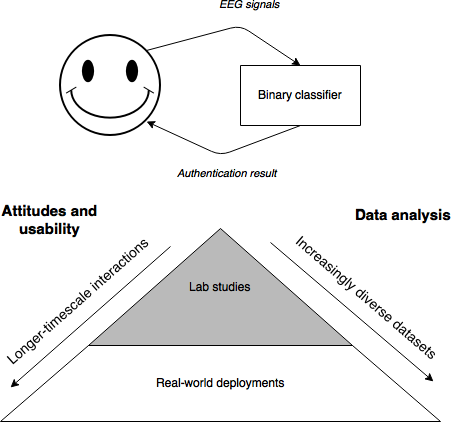
\includegraphics[width=.9\linewidth]{./figures/passthoughts-diagram.png}
\caption{Challenges moving passthought authentication from the lab to the real world.}
\end{figure}


While recent work is heartening, passthoughts remains confined, for now, to the lab.
This paper reviews the immediate questions that must be addressed if passthoughts is to move into everyday life (Figure \ref{fig:diagram}).
First, we must understand the real usability properties of passthoughts.
The usability of passthoughts authentication will depend not only on its performance in ecologically valid contexts,
but also on people's attitudes about brainwaves, EEG, and biosensing generally (Section 3).
Second, we must test passthoughts in a variety of conditions: ambulatory settings, under different levels of stress, drowsiness, caffeine or alcohol, etc.
This statistical analysis will help us understand 
the space of possible passthoughts,
and how passthoughts change over time (Section 4).

In addition, computing broadly has undergone many sea changes since passthought's initial proposal in 2005.
Biosensing (the sensing of humans) has proliferated throughout our everyday life, due both to the sensors ubiquitous in smartphones, and to general improvements to infrastructures of data collection and machine learning at scale. 
Is passthoughts more or less appealing in light of other authentication strategies these "sea changes" have made possible? 

This paper aims both to re-validate passthought's promise as an authentication paradigm (Section 2), and to 
motivate and contextualize two studies that could begin to address the challenges posed above (Section 5).
While passthoughts is not without risks (Section 6),
it could lead to novel \emph{types} of authentication,
which challenge (or at least destabilize) dominant assumptions about what authentication 
can and should be able to do. (Section 7).

\section{Background}
\label{sec:orgf24757b}

Authentication seeks to prove that a user is who they claim to be.
In computer security, authenticators are classified into three types: knowledge factors (e.g., passwords
and PINs), possession factors (e.g., physical tokens, ATM cards), and inherence
factors (e.g., fingerprints and other biometrics). 

An ongoing problem in authentication lies in balancing strong security
(i.e., multiple factors of authentication)
with usability.
As an example, major industry players such as Google and
Facebook have strongly encouraged their users to adopt two-factor
authentication (2FA), in which a user enters his or her password (a knowledge factor),
and subsequently receives a code on their cellphone (a posession factor).

However, submitting two different 
authenticators in two separate steps has frustrated wide adoption
due to its additional hassle to users. The Apple iPhone, for instance,
already supports device unlock using either a user-selected passcode or a fingerprint. The
device could very well support a two-step two-factor authentication scheme if
desired. However, it is easy to understand why users would balk at having to
enter a passcode \emph{and} provide a fingerprint each time they want to unlock their phone.

To assist with the usability issues surrounding multi-factor authentication,
passthoughts aims to provide two factors of authentication in a single step.
A single mental task, or passthought, provides both a knowledge factor (a chosen secret thought)
with an inherence factor (the way that thought is expressed for an individual) \cite{Chuang2013b,Johnson2014}.
Using a custom sensing device, passthoughts could provide an additional posession factor, all in the same step.


\subsection{One-step, multi-factor authentication}
\label{sec:orgc869159}

Since passthought's initial proposal in 2005,
more ubiquitous sensing and computing has enabled a number of other strategies for achieving two factors of authentication in a single step. 
Some work has tested behavioral authentication methods such as keystroke dynamics, or voice. In both cases, the knowledge factor (password or passphrase) and
inherence factor (typing rhythm or speaker's voice) are employed \cite{Monrose1997}.
In contrast, the Nymi band supports one-step two-factor authentication via the inherence
factor (cardiac rhythm that is supposed to be unique to each individual) and the
possession factor (the wearing of the band on the wrist) \cite{Nymi}.
More recent attempts have also used gait (from cellphone accelorometers) to perform authentication \cite{UnifyID2017}.

However, these existing strategies are susceptible to a variety of attacks. 
Nymi, for example, does not have a knowledge factor, making it impossible for the user to change the authentication token if the device and biosignal have been compromised.
Keystroke dynamics, voice, and gait are all susceptable to ``shoulder surfing,'' in which an attack uses visual or other cues to steal, or improve the chances of guessing, a target's chosen secret. 
Passthoughts mitigates this attack by nature of the mental gesture.
Since the expression of a passthought is not externally visible, the authenticator is impervious to shoulder surfing attacks.
Since the thought a chosen secret (knowledge factor), it can be changed if compromised. 

\subsection{Passthought authentication}
\label{sec:org59cf6e1}

The use of EEG as a biometric signal for user authentication has a short history.
In 2005, Thorpe et al. motivated and outlined the design of a passthoughts system \cite{Thorpe2005}. Since 2002, a number of independent groups have achieved low (less than 1\%) false acceptance rates using multi-channel sensors placed on the scalp \cite{Poulos2002,Marcel2007a,Palaniappan2008,Ashby2011}.
In 2013, one group showed that similar accuracy can also be
achieved using a consumer-grade single-channel sensor \cite{Chuang2013b}. 
In particular, the lack of signal diversity from multiple EEG channels can be overcome by allowing
the users to choose their own personalized passthoughts (e.g., sing their favorite
song in their head). There are two significant consequences of this result. First,
the passthoughts approach is no longer constrained by the high cost (> \$10,000 USD)
and low usability (gel-based electrodes; aesthetic challenges of an EEG cap) of
medical-grade multi-channel devices. Second, because users can choose and
easily change their secret mental task, this approach can support one-step two-
factor authentication via the simultaneous presentation of the inherence factor
(brainwave signatures due to the unique folding structures of the cortex) and the
knowledge factor (the secret mental task) \cite{Chuang2014}.

\subsection{Passthoughts using in-ear EEG}
\label{sec:orgf65c549}

Even consumer-grade headsets can be uncomfortable to wear, and are awkwardly visible to outside observers. 
Earbuds present a more discreet, comfortable location for an EEG sensor, as earbuds are already commonly worn.

\label{fig:earbud}
\begin{figure}[t!]
\centering
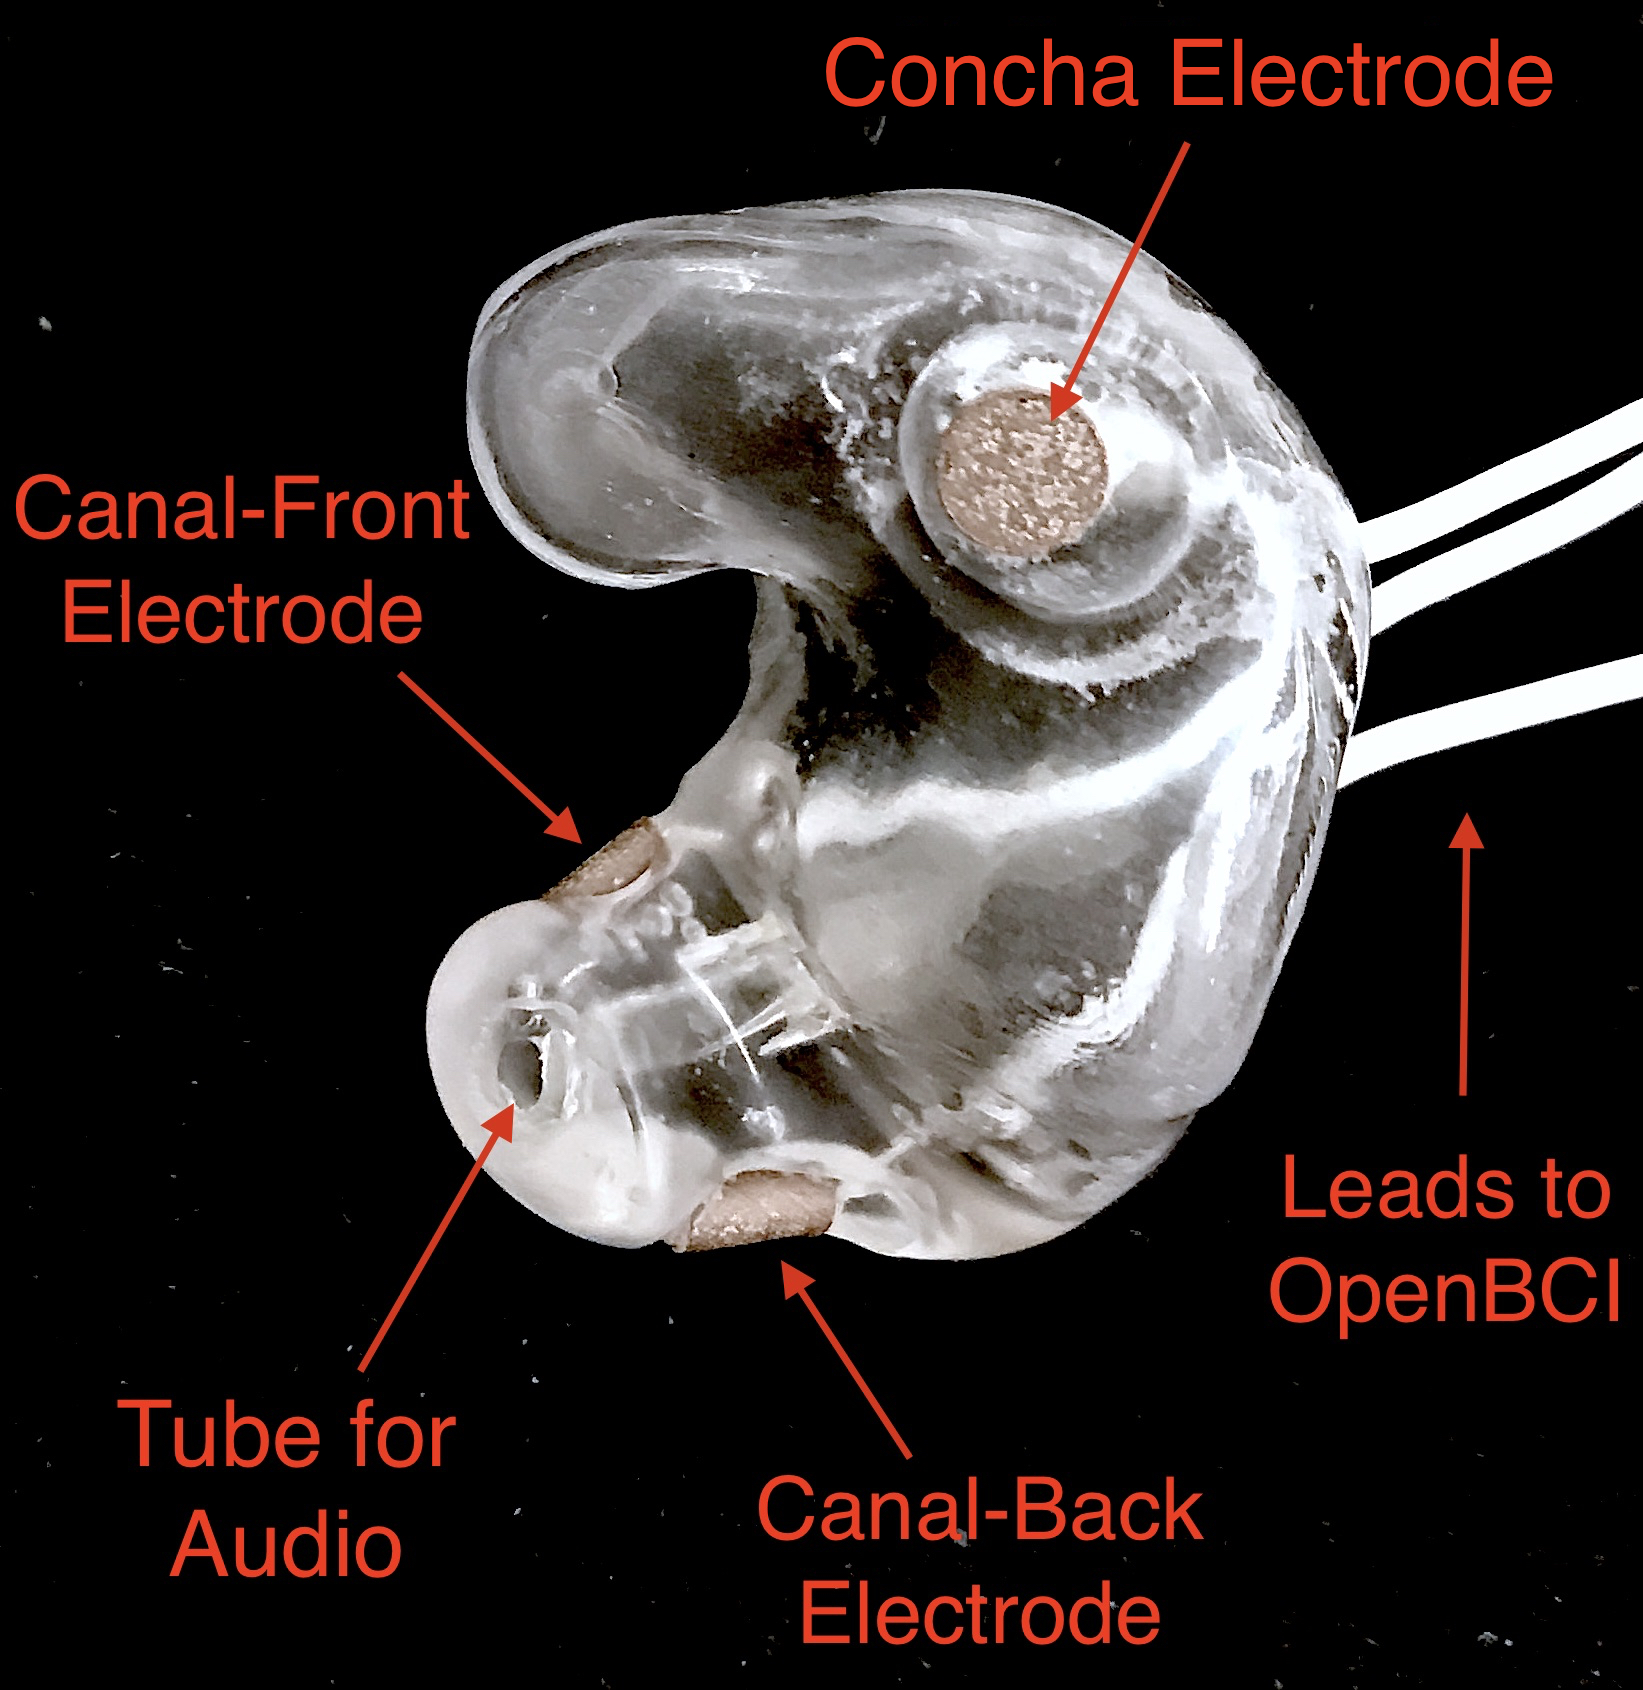
\includegraphics[width=.9\linewidth]{./figures/custom-fit-eeg-annotated.jpg}
\caption{A custom-fit in-ear EEG device as used in Curran et al, 2017}
\end{figure}

Research in in-ear EEG is only several years old. Nonetheless, the concept has
attracted a lot of attention because of the discreetness factor of in-ear EEG over
traditional scalp-based EEG. A research team at the Imperial College London
and Aarhus University published a landmark paper in 2011 that introduced the
concept of in-ear EEG, demonstrating for the first time the feasibility of recording
brainwave signals from within the ear canal
\cite{Looney2011}.
Follow-up work from the same
group demonstrated its ability to produce signal-to-noise ratios comparable to
those from conventional EEG electrode placements, robustness to common
sources of artifacts, and use in a brain-computer interface (BCI) system based on
auditory evoked potentials and visual evoked potentials
\cite{Looney2012a,Kidmose2013a,Kidmose2013b}.

The first attempt to merge in-ear EEG with passthought authentication
used a modified consumer grade EEG device with a single electrode, achieving approximately 80 percent authentication accuracy \cite{curranpassthoughts}.
Ongoing work from the same authors investigates the use of custom-fit earbuds with multiple embedded electrodes \ref{fig:earbud}.
Lending credibility to that study's claim that in-ear EEG could one day become feasible in consumer devices,
United Sciences recently announced a consumer "hearable'' (in-ear wearable) called The Aware, which will measure EEG from the ear, among other biometrics.

\section{User attitudes and perceptions}
\label{sec:orgd0ec90a}

While past work makes passthoughts less visible with more discreet form-factors,
a large question still remains:
What sense would people make of passthoughts, as a technology, in their everyday life?
This question begs not only user-centered design studies with passthoughts itself,
but more general questions about what EEG means to people,
and what people believe EEG data can reveal about them.
Past work has established that people tend to ascribe almost magical abilities to brain-scanning devices, even subjects with specific training in the limitations of brain-scanners \cite{Ali2014a}.
Will these attitudes scare away, or attract wider adoption?
This section outlines common concerns around ``mind-reading'' machines, and how they relate to EEG and passthoughts specifically.

\subsection{Contending with mind-reading machines}
\label{sec:org070ba38}

Biosensing devices in general raise many questions about privacy for end-users,
typically around the meaning of the data produced by particular devices.
For example, you might be eligible for an insurance discount if you wear a FitBit \cite{Bernard2015} (depending, of course, on what readings the FitBit produces \cite{Brain2015}). 
But, would you wear a device in the workplace \cite{solon2015}, if your manager used it to track your productivity?
If biosensor data can be used in the courtroom \cite{Crawford2014}, could not pervasive biosensing help to \emph{predict} crime \cite{Thompson2011}? 
After all, one study suggests that probability of involvement in violent crime can be predicted from one's resting heartrate \cite{Latvala2015}. 
In all of these examples, biosensing technologies blur the line between \emph{sensing bodies} and \emph{sensing minds}. 
Now, when people decide to buy sensor-equipped consumer devices \cite{Stables2016}, or get sensed passively by devices integrated into the walls and ceilings \cite{Adib2015} or city streets \cite{Thrift2014}, end-users will need to contend with the prospect of mind-reading machines.

If people \emph{think} a certain technology measures aspects of mind, it will certainly affect the way they engage with that technology, 
whether or not it works the way they expect \cite{Ali2014a}. 
Meanwhile, if they think that a given technology does \emph{not} measure their mind, when in fact it does, users may suffer a breach of what Nissenbaum might call the ``appropriateness of the flow of information'' \cite{Doyle2011}. 
In both cases, knowing what people expect will help us anticipate their needs and concerns.

If we wish to understand what role passthought authentication \emph{could} play in day-to-day life,
we must view it both through the lens of potential privacy concerns, \emph{and} through the lens of possible opportunities for self-reflection and self-understanding. 
Of course, users' attitudes will not be fixed: they will evolve over time, as users observe the device in action, and correlate its judgments with their own lived experiences \cite{Nafus2016}.
In the next section, discuss how EEG as a sensing modality motivates questions around the meaning people may build around passthought authenticators.


\subsection{What (do you think) EEG can reveal about a person?}
\label{sec:orgecc4d41}

The survey we report on here, currently in-progress, examines how people's beliefs differ given device ownership, and their membership in one of two groups: Mechanical Turk workers, or people enrolled in Health-e-Heart, a massive (n > 40,000), longitudinal study, in which volunteers fill out surveys about themselves, and/or upload data from biomedical self-tracking devices, over the course of several years \cite{Estrin2010a}.
In one portion of the survey, we ask subjects to rate a number of different biosensors in order of how likely individual's believe each sensor is to reveal what ``a person is thinking or feeling'' (Figure \ref{fig:rank}).
This section reports on a subset of Mechanical Turk workers (n=100) and Health-e-Hearth subjects (n=100).

In our preliminary findings, brainwaves (EEG) are seen as among the most revealing biosignals, just below body language and facial expression, in their capacity to reveal the goings on of a person's mind. 
More common sensors such as GPS and step count are seen as less revealing (despite empirical evidence suggesting such data can be quite revealing indeed \cite{Canzian2015}).
What will this finding mean for wider adoption? 
Will people shy away from using their passthought authenticator in certain situations, or when they are feeling some type of way?

\label{fig:rank}
\begin{figure*}
\centering
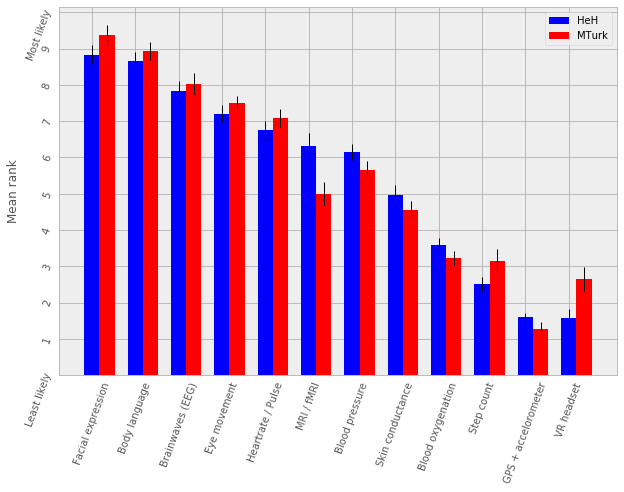
\includegraphics[width=.9\linewidth]{./figures/rankings.png}
\caption{``Please rank the following sensors in how likely you believe they are to reveal what a person is thinking and feeling.'' Higher bars indicate higher rank, or higher likelihood of being revealing.}
\end{figure*}

Our qualitative data revealed that subjects in both groups generally believed EEG to reveal various details about the mind, mood, emotions, and identity.
We asked subjects to reflect on why they answered the way they did during the ranking task (Figure \ref{fig:rank}).
In the Health-e-Heart group, several subjects gave relatively specific explanations as to why they ranked EEG hihgly.

\begin{quote}
\emph{(S24) I assume some information can be gleaned from brain wave activity in various parts of the brain related to rewards or executive control, but without accompanying information, it may be difficult to discover my thoughts.}
\end{quote}

\begin{quote}
\emph{(S23) EEGs note parts of the brain that are active.  Again, in conjunction with other measurements, I suspect that some sense of what one is thinking and feeling could be learned.}
\end{quote}

\begin{quote}
\emph{(S91) I would rate this relatively high on the list because science has shown that we can detect a lot about which areas of the brain are accessed and at which times.  This can tell a person a lot about what they might be thinking and especially how they are feeling.}
\end{quote}

While these explanations range somewhat in their specificity and confidence,
they share the general sentiment that EEGs can be revealing. Subjects in the Mechanical Turk condition broadly shared this belief, though tended to use less physiological detail in their explanations.

\begin{quote}
\emph{(S157) Brain activity can pinpoint exact emotions by monitoring certain areas on the brain.}
\end{quote}

\begin{quote}
\emph{(S130) Brainwaves could tell you a lot more about what someone is thinking and feeling. You could measure the patterns of brainwaves in an experiment.}
\end{quote}

Meanwhile, some subjects from both groups did not fit this trend. Ten subjects ranked EEG low in its ability to measure what a person is thinking or feeling. Their qualitative answers revealed a diverse set of reasons for this ranking.
Three subjects indicated a general lack of faith in brainwave's reliabilty.

\begin{quote}
\emph{(S20) I don't think we have the ability to translate brainwaves into thoughts or emotions.}
\end{quote}

\begin{quote}
\emph{(S101) EEG is very nonspecific and rarely can tell details reliably.}
\end{quote}

\begin{quote}
\emph{(S138) Possible but not accurate.}
\end{quote}

These explanations broadly centered around EEG as a signal.
They range somewhat in their confidence, from a fundamental skepticism (S20) to caveats about possible accuracy or specificity (S101, S138).
In contrast to these three subjects, S10 ranked EEG low because s/he
felt the premise of a consumer grade EEG was implausible.

\begin{quote}
\emph{(S10) I assume that scientists can identify by brain patterns what others are feeling and thinking based off of years of research.  I've never heard of a consumer grade eeg - and doubt it could be as powerful as a laboratory eeg.  If it is then I would be interested in this product.}
\end{quote}

This subject's explanation surfaces the practical differences in attitudes that people might have to a technology's theoretical existence,
and its realized existence as a consumer device. Future work could look more closely at 
how the presumed scientific authority of a brainscanning apparatus affects people's willingness to accept specific BCI applications such as passthoughts \cite{Ali2014a}.
Finally, one subject's skepticism what brainwaves can reveal stemmed from his/her personal medical experiences.

\begin{quote}
\emph{(S116) My son has absence seizures, so his brainwaves change.}
\end{quote}

This quote highlights how individuals' life experiences
might shape the way they engage (or refuse to engage) with brain-sensing devices.
In general, this quote and others motivate the need for a rich, qualitative understanding of people's first-hand experiences with brainscanning devices,
as well as data collection,
in order to understand what role BCI applications such as passthoughts could play in day-to-day life.
\section{Diversity and security of passthoughts}
\label{sec:org2322423}

While the previous section outlined questions around user attitudes, empirical questions about passthoughts, as signals, also linger.
This section outlines and motivates the major quantitative questions that have not been fully answered by past work on passthoughts.

While past work on passthoughts has achieved excellent results using recordings from different users, 
these studies do not consider a variety of different subject conditions.
For example, sitting subjects may have different patterns of neural activity from subjects who are standing, walking or exercising \cite{Thibault2016a},
let alone subjects who are under the influence of e.g. caffiene or alcohol.
Passthoughts studies must collect larger, and more diverse corpora of EEG data to examine how passthoughts change (or remain stable) throughout the dynamic contexts of daily life.

Investigating this topic could also help us understand how and why passthoughts work at all: Why are passthoughts unique, and how unique are they?
A primary question in passthoughts surrounds how large the real space of possible passthoughts might be \cite{Thorpe2005}.
While the space of possible passthoughts is potentially unlimited, we do not yet know what passthoughts we stand a reasonable chance at observing consistently over time.
A larger corpus of data might help shed light on this issue by allowing us to observe the distribution of signals that people produce over time.

A more subtle, but related question surrounds how passthought EEG recordings compare to non-passthought EEG recordings.
In other words, we do not know how the particular passthoughts observed in past work are drawn from the distribution of EEG signals that an individual produces over the course of their day.
This blind-spot poses a possible challenge to passthought's vulnerability to dictionary-style cracking.
If an attacker has a large enough corpus of EEG readings, do some passthoughts start to look as guessable as \emph{password1234}?
By answering such questions, we could design data-driven policies for, e.g., how many retry attempts passthought authenticators should allow.

\section{Two studies on passthoughts}
\label{sec:orgfeb449a}

The prior two sections raise two main topics that future work could address. 
First, our limited understanding of passthoughts' usability, and user attitudes about the sensing modality present immediate questions for further development of this technology.
Second, our limited knowledge of how passthoughts shift and change over time, and around the diversity of EEG signals as our (non-medical) devices sense them,
raise questions about how frequently passthoughts would need to be calibrated, how accurate we can expect the protocol to be in different context, and how secure it might remain under threat from a motivated attacker.

This section proposes two studies on passthought authentication which, taken together, could make headway on these topics.
One study, a controlled, lab-based experiment, seeks to raise fundamental questions about how the feedback of a real-time authentication system may affect the way users perform their passthoughts.
It also begins to address certain, limited questions around the shifting nature of neural signals.
The second study, a longitudinal deployment, seeks to collect a large and diverse corpus of EEG signals, while probing people's beliefs and attitudes about EEG and brainscanning in everyday life.
Together, these studies address both long-term concerns about user attitudes and signal diversities, and also short-timescale questions about the usability and accuracy of passthoughts in realistic use scenarios.

\subsection{A real-time passthought authenticator}
\label{sec:org9b0d095}

Passthoughts promise more usable form multi-factor authentication compared to existing protocols,
as they provide both a knowledge and an inherence factor in a single-step user action.
However, no study yet has systematically evaluated passthoughts' usability.
Here, we propose a study aimed at examining passthoughts' usability in an ecologically valid context.

\subsubsection{Study protocol}
\label{sec:orgbdaa522}

This study would take place in a lab, under the supervision of an experimenter.
First, the experimenter would calibrate a subject with a passthought authenticator, as in \cite{Chuang2013b}.
Through an automated cross-validation process, the participant's best-performing passthought would be selected.
Next, the experimenter would present users with an online banking application, and ask them to perform their passthoughts.
We can manipulate feedback such that users either see the real authentication accuracy (control), 
are always rejected by the authenticator, 
or always accepted by the authenticator.

After this task, subjects could take a post-questionnaire including various usability questions.
After filling out this questionnaire, the experimenter might engage users in a brief, ten-minute semi-structured interview,
in which subjects are asked to recount their experience with the authenticator.
This interview could help gain some richer, qualitative data that traditional survey methods might fail to capture.

\subsubsection{The effect of feedback}
\label{sec:orge6fa888}

Through this study, we might find 
that passthoughts is considered usable, even when authentication attempts are always rejected.
We might also find that passthoughts are not considered usable, 
even when authentication attempts are always accepted.

Furthermore, using the data collected during this study, we could perform an offline analysis 
to test for the effect of these conditions on the actual performance of users' passthoughts.
When subjects are continuously rejected, do their passthoughts change in frustration (or in an attempt to gain access)?
We might find that passthought performance 
remains stable, regardless of what feedback subjects are shown.
Alternatively, we might find that performance changes 
when subjects are continuously rejected from their authenticator.
Alternatively, performance may change, 
even when subjects are continually accepted by their classifier.

This study's findings could have far-reaching impacts for the future development of passthought authenticators.
Its results would shed light on how passthoughts change as a response to authenticator performance on one hand,
and how authenticator performance affects perceptions of passthoughts' usability on the other.

\subsubsection{Exploring continuous re-calibration}
\label{sec:org1b70139}

In addition to these findings, the data generated during this study could help test 
a third hypothesis: that the continual re-training of passthought classifiers might help boost classification performance over time,
especially in the face of shifting signals.
Offline, we can train each classifier, for each subject, to achieve its post-calibration state.
Next, we can run each reading recorded from a particular participant through the trained classifier.
If the classifier accepts the reading, we can then re-train the classifier, 
adding this reading to the corpus of positive examples.
In a separate, \emph{negative calibration} condition, 
we can also re-train the classifier with rejected readings as negative examples.
This condition should reduce false acceptances from the target subject, re-inforcing our authenticator's knowledge factor.

By comparing the final FAR and FRR for each subject using these strategies, 
compared to the one-time calibration strategy, we could begin to get an idea as to whether
this strategy helps achieve superior performance, especially when signals change.
This analysis could also act as a harbinger for some of the possible downsides of this approach:
If a user is continually rejected, and the classifier is re-trained using those rejections as negative examples,
will the user find themselves trapped in a negative spiral of ever-decreasing authentication accuracy?

\subsection{A longitudinal study on brainwave monitoring}
\label{sec:org89ebd65}

The study proposed above would help answer preliminary questions about
the usability of a passthought authenticator in a short-term context,
and possible ways for dealing with shifting neural signals,
a few questions will still remain.
First, the study above will not help us collect a large corpus of EEG signals, 
preventing us from investigating how robust passthoughts authentication performs in various user conditions,
and from understanding how easy particular passthoughts are to guess or crack.
Second, while the previous study helps us understand user attitudes over a short timescale,
it will not help us understand how people's beliefs about EEG might change over longer periods of time, as they use their devices in day-to-day life.

Unfortunately, these challenges (particularly those around shifting neural signals) also make it difficult to produce a passthought authenticator that works with any reliability in real-life contexts.
This makes a longitudinal study with a working authenticator impractical for the time being.
However, we may still perform a longitudinal study that allows us to interrogate the usability aspects around (and attitudes about) passthoughts specifically, and EEG generally.
In so doing, we may also collect a larger and more diverse corpus of passthoughts, which can be used to address the paucity of data we face today.
This section describes a technology probe \cite{Gaver1999} that could help address both of these issues at the same time.

\subsubsection{Study protocol}
\label{sec:org51af8ed}

A small group of subjects could wear a working, recording EEG device, whether or not it provides feedback, in a variety of settings for some number of days,
having subjects journal their experiences and asking them specifically what they feel someone might be able to know about them from the EEG signals they record.
At the same time, we could use this study as an opportunity to collect a much larger, and more diverse corpus.
To aid in the collection of signals that are specific to our problem of passthought authentication,
subjects in this study might be prompted to perform a variety of tasks at a few checkpoints throughout the day.
With the data collected during this study, we could easily simulate passthought accuracy on a much more realistic (and representative) sample of readings.

Such a study would trade a large population size for a large corpus of diverse data.
This tradeoff allows us to closely investigate the diversity of EEG signals within subjects.
The diverse readings encountered in day-to-day life could help us understand how such signals change as a function of time, and/or in different psychophysical states.
At the same time, our user diaries and interviews could enable a rich, qualitative understanding of users attitudes.

\subsubsection{A more diverse corpus}
\label{sec:orgabae915}

While subjects wear their EEG device and diary about their experience, we should also ask subjects to perform
targeted mental tasks (potential passthoughts) in a variety of contexts (ambulatory, under the influence of caffeine or alcohol, etc). 
This diverse corpus should allow us to both evaluate performance in ambulatory settings, and to
investigate the possibility that past works' models overfit for subjects who are sitting down in a lab.
How do an individual's EEG signals change throughout various activities, and mental states?

This corpus will, of course, also include unlabeled non-task data from similarly diverse settings, perhaps concurrent with streams of GPS or accelorometer data.
Unlabeled data represents another fruitful source of data for passthoughts.
The unlabeled samples in this corpus also allow us to examine properties of EEG signals in general, helping us build more robust models which should help us prevent overfitting in the future.

\subsubsection{The space of possible passthoughts}
\label{sec:orgf932e18}
In another potentially fruitful analysis, such a corpus will allow us to perform statistical analysis of how passthoughts are drawn from the overall distribution of EEG signals. 
Using multi-dimensional clustering algorithms such as t-SNE \cite{VanDerMaaten2008} 
could assist us in understanding how particular passthoughts relate to other EEG signals that an individual expresses involuntarily throughout the day. 
These clusters will help us understand how likely or unlikely we are to observe a given passthought in context of a particular person's neural signals
Such analysis between subjects could help shed light how given passthoughts are expressed uniquely between individuals.

Leveraging the statistical clusters of EEG data generated by these algorithms, it might also be possible to generate a ``passthoughts cracker,'' capable of generating plausible passthoughts. 
Feeding these algorithms into pre-trained passthought classifiers, we can begin to generate realistic models of classifiers' resistance to cracking attempts. 
These cracking experiments could lead to defenses against cracking attempts, by enforcing retry attempt timeouts or other methods for limiting break-in risk, such that strong security guarantees can be enforced.

\subsubsection{Usability and attitudes}
\label{sec:orge48f8f8}

By deploying a real sensing apparatus, be it a traditional consumer device such as the Muse \cite{Mihajlovic2015} 
or a more experimental piece of equipment such as an earbud,
and having people record EEG data in their daily life, we could learn more about the interpretative qualities of these data \cite{NafusDawn;Sherman2014}.
This study presents a dual opportunity to understand user beliefs with rich, qualitative data, 
while simultaneously collecting the large, diverse and longitudinal corpus of EEG signals necessary if we wish to stand a chance at decent authentication accuracy in the wild.

\subsubsection{Limitations}
\label{sec:org32c6e47}

This study would be no substitute for a working, online passthoughts authentication system.
Instead, this study aims to collect useful data before such a system exists.
It will not only elicit beliefs, 
but also allow us to collect larger datasets, 
and to catch technical issues in sensing devices and collection platforms.

Even in this goal, the proposed study has a few limitations.
First, it is unclear how closely the study protocol maps to actual passthought use in the wild.
For example, people who use passthoughts may not wish to wear an EEG device all day, as our subjects would.
Furthermore, the system proposed here does not provide a realistic authentication context, in that subjects
are asked to use the system at pre-defined points during the day. 
Future work could create more realistic concepts, perhaps ones in which subjects have an intrinsic motivation (or stake) for the authenticator to work correctly.

\section{Privacy, Security: Choices, Tradeoffs}
\label{sec:org8f30435}

After the studies described above, 
we will have a much better grasp on the usability, and security properties of passthought authentication.
However, there may still be unexplored risks, challenges, and tradeoffs,
especially around user privacy.
Indeed, some of these risks are unique to the application context of biometric authentication, and to EEG as a class of biosignal. 
This section briefly reviews risks to user privacy and security that widespread passthought authentication may introduce. 
We present broad class of categories from which such risks may emerge. 

\subsection{Privacy}
\label{sec:org792897a}
As of yet, it is still not well understood what EEG signals might reveal about a person.
EEG signals that are not anonymized could come to be seen as private in the face of new methods of analysis.
(If your brainwaves can authenticate you, could they also uniquely identify you, even if your name is redacted?)
Differential privacy \cite{Dwork2014} presents one approach to dealing with the risk of privacy breaches with EEG signals.
By adding noise to datasets, differentially private databases can make strong guarantees about the likelihood of a de-anonymization attack on particular database queries.

\subsection{Security}
\label{sec:org9f1d640}
Device security presents another risk to passthought authentication.
Since EEG devices will transmit data, likely wirelessly \cite{Mihajlovic2015}, their data may be intercepted, depending on the security properties of the underlying transit protocol. 
When transferring authentication credentials in passthoughts, the ability to snoop on authentication attempts could present a dangerous attack vector.

There is also the question of the security of data infrastructures in which EEG data might be stored.
Large data repositories are what Wolf \cite{Wolf2010} calls a ``toxic asset''; they must be maintained, 
lest the maintainer take liability for harmful fallout of poor data management.
With biosignals, it is not always clear what they might mean until they are already collected in aggregate. 
By then, it is too late to decide on an appropriate data security policy.

Strong encryption policies should be built into collection systems from the very beginning, 
It remains an open question what specific protections and access controls will yield robust security.
Homomorphic encryption, in which computation such as database queries can be performed on encrypted data, provides one interesting path for future work \cite{Tu2013}.

\subsection{Tradeoffs between security and privacy}
\label{sec:orge87f2fc}

In some cases, passthoughts could present direct tradeoffs between security and privacy.
For example, end-user privacy could be enhanced by storing all data locally, on the phone. 
All classification, and the training of all classifiers, could occur locally, so that users never need to disclose their private biosensory data to a third party.
However, security might be improved by aggregating user data so as to construct more robust, reliable classifiers.
Aside from classifier accuracy, training classifiers in the cloud could help with the speed of calibration,
and prevent undue battery drain on user devices.

These factors suggest a possible tension between the accuracy (and thus security) of passthought authentication,
and the locality (and thus privacy) of potentially sensitive user data.
Future work should explore this tradeoff empirically, using real data and simulations from a variety of different users.
Future work might also explore metrics by which to judge such tradeoffs.
Whereas security might be measured straightforwardly using false-acceptance and false-rejection rates,
user privacy might be more challenging to quantify, as might the tradeoffs between the two.
However, future work will need to address these issues if we are to balance users' security requirements with their privacy requirements.

\section{Further Future Directions}
\label{sec:orgce50b86}

This paper so far has motivated two future studies on passthoughts,
and discussed potential risks intrinsic to the development of passthoughts systems.
With these risks in mind, the present section explores some of the exciting possibilities that could unfold after the immediate priorities described in the prior sections.
Through the lens of passthoughts, we hope to use this discussion as an opportunity to challenge (or at least destabilize) dominant assumptions in authentication.

\subsection{Continuous authentication}
\label{sec:orgd749d30}

After immediate challenges are overcome,
one potentially exciting possibility is that of using EEG for \emph{continuous authentication}.
Continuous authentication schemes seek to authenticate a user using ongoing streams of data or activity, sometimes by giving a probability that a person's identity is authentic \cite{Bojinov2012}.
Such schemes are a natural match for wearables, which can continuously collect and process biometric data.
A recent startup, Unify.ID, has begun to perform cross-device continuous authentication as a service \cite{UnifyID2017};
however, as a knowledge factor, it currently falls back on traditional passwords, which come with both well-known risks and annoyances to usability.

A continuous passthought authenticator could incorporate both knowledge and inherence factors (along with, optionally, the posession factor of a unique sensing device).
Subjects could perform secret passthoughts for certain unlocking actions,
while the authenticator could fall back on inherence in the base case (e.g. as an additional check on sites where the user's logged-in session would otherwise be remembered).
In theory, this strategy provides better security properties than saved sessions or cookies, 
which, after initial authentication, establish only posession. 
Individual login attempts also offer security improvements over traditional passthoughts alone, as the continuous inherence step provides an ongoing validation against individual authentication attempts.

\subsection{Organic passwords}
\label{sec:orgdc73e84}

If EEG signals are nonstationary (changing over time), passthoughts will require continuous re-calibration to maintain decent accuracy \cite{Vidaurre2006a}.
This feature of BCIs could have an unexpected benefit to security. 
If an individual's expression of their passthought in EEG is always changing, 
passthoughts themselves are effectively evergreen, automatically replaced or updated by nature of the authentication paradigm.
This feature could improve security, as an attacker able to compromise a passthought's EEG signature may not be able to log into the system in a few weeks time,
unless they are able to realistically mutate the signal over authentication attempts.
This feature of EEG also gives passthoughts a possible advantage over other methods for behavioral authentication, such as voice or keystroke dynamics \cite{Monrose1997}, which may change more slowly for individuals, if they change at all.
Future work should investigate this claim, perhaps using a longitudinal corpus such as the one described above.
\subsection{Authentication and the self}
\label{sec:org1391488}

Where authenticity is nominally concerned with proving that you are who you say you are,
a less-frequently-asked question in the authentication literature is,
``are you really yourself?''
We all sometimes do or say regrettable things when we are feeling ``not quite ourselves,'' sometimes using devices or services with which we have authenticated ourself.
Can authentication ever verify not only your possession of your body, but of your ``right mind''?

A question raised earlier surrounds where passthoughts could still work if a person is drunk, having a migraine, or in distress (Section 3). 
Even if passthoughts fails when a user is in such an ``off-baseline'' state, 
passthoughts still may have utility (perhaps even \emph{added} utility) in certain authentication contexts.
For example, one may wish to allow themselves access to certain resources (e.g. bank accounts) when one's resting EEG state is not too much different from a pre-recorded baseline.

Such a scenario raises serious ethical, legal, and even philosophical questions. 
How does such a system conform to accepted definitions of a ``person''?
Who is a person to make decisions for their future self?
What are possible vectors for abuse?
In any case, this property of an authentication is, as far as we are aware, novel, 
and should be considered as we learn more about the strengths, weaknesses, and particular affordances of this developing method for authentication.
\subsection{Passthoughts by any other sensor?}
\label{sec:orgdfab018}

At the end of the day, past passthoughts work has collected electromagnetic signals from the body at the surface of the skin.
What is important about passthoughts is not so much the EEG per se, but that it is both secret and idiosyncratic (knowledge and inherence), that its performance had no tell, and that its performance was not easily explained to others.
EEG itself brings a variety of challenges: it is a low-magnitude signal, prone to noise, and inconvenient to capture without special equipment.

There is no theoretical reason why the same criteria cannot be met with, e.g., EMG from the face, or a mixture of EEG and EMG.
Muscular activity associated with thoughts might, after all, be both difficult to view and consistent between trials.
Future work could investigate such claims further, or use different types of sensors that may have a similar effect (EKG, fNIRs).

\subsection{Health, neuroscience and BCIs}
\label{sec:orgfdf7b6f}

Neuroscience fuels some of the most chilling predictions in science fiction \cite{Welsh2011}.
It also stands for some of the greatest possible advances in medicine, mental health, and understanding of human behavior.
One ambitious goal is to detect or even predict seizures \cite{Mormann2006}.

However, the original, and most active areas of research in BCI surround the creation of tools for persons with muscular disabilites \cite{Carrino2012}.
By collecting unstructured or semi-structured EEG data in the wild, passthought systems could help improve the development of such BCIs \cite{Grierson2011a}.
The small size of data repositories, limited mostly by the clinical trials needed to build BCIs for persons with disabilities,
has consistently frustrated attempts to improve on algorithms and protocols in this field \cite{Allison2009}.

Though the application context for passthoughts is quite different from wheelchairs,
and although passthought users may not have muscular disabilities,
pursuing passthoughts as an area of research will inevitably yield larger repositories of EEG data than have been collected to date.
This data could prove invaluable for the development of EEG-based BCIs across a variety of fields, including (but not limited to) assistive technologies.

Again, these opportunities must strike a balance with the risks of individual users' privacy and security.
Violating user privacy by revealing EEG data, even to researchers, could undermine any chance of wider BCI adoption in the long-term.
Striking this balance will require a deeper understanding of the statistical properties of signals. 
How much data will users really need to give up? 
What counts as an ``anomalous'' reading?
Answers to these questions could themselves inform neuroscientific inquiry.
This balance will also require a deeper understanding of individuals' attitudes about the meaning of such signals,
and how private people believe them to be.

\section{Conclusion}
\label{sec:orga0b4a2b}

In general, as sensors grow smaller and cheaper, devices more connected, and machine learning more sophisticated, 
people will build increasingly high-resolution models of human physiology ``in the wild.''
Passthoughts present just a microcosm of the good such advances might bring, 
along with some of the most pressing anxieties: 
What does pervasive physiological recording mean for our privacy, security, safety? 
The balancing act between these risks and opportunities will prove recurring theme for decades to come.
In the meantime, probing the outer limits of ubiquitous, pervasive sensing can shed light on both the good and bad that our near future may bring.

\bibliographystyle{ACM-Reference-Format}
\bibliography{refs}
\end{document}
